\documentclass{article}

\usepackage{ctex}
\usepackage{van-de-la-sehen}

\begin{document}

\section{各种坐标系} % (fold)
\label{sec:各种坐标系}

\subsection{二维正交坐标系} % (fold)
\label{sub:二维正交坐标系}

\subsubsection{椭圆坐标系} % (fold)
\label{ssub:椭圆坐标系}

\begin{figure}[ht]
    \centering
    \includegraphics{src_plot/Elliptic.pdf}
\end{figure}

\paragraph{坐标曲线} % (fold)
\label{par:坐标曲线}

共焦的椭圆与双曲线. 通常设两个焦点为$\pare{\pm a, 0}$.

% paragraph 坐标曲线 (end)

\paragraph{转换关系} % (fold)
\label{par:转换关系}

与平面直角坐标系有转换
\begin{align*}
    x &= a\cosh \mu \cos \nu, \\
    y &= a\sinh \mu \sin \nu.
\end{align*}
其中$\mu \ge 0$, $\nu \in \lbr{0,2\pi}$.

% paragraph 转换关系 (end)

\paragraph{度规} % (fold)
\label{par:度规}

\begin{align*}
    h_\mu &= h_\nu = a\sqrt{\sinh^2 \mu + \sin^2 \nu} = a\sqrt{\half \pare{\cosh 2\mu - \cos 2\nu}},\\ \rd{A} &= a^2\pare{\sinh^2\mu \sin^2\nu}\,\rd{\mu}\,\rd{\nu}.
\end{align*}

% paragraph 度规 (end)

\paragraph{微分} % (fold)
\label{par:微分}

\begin{align*}
    \laplacian \Phi = \rec{a^2\pare{\sinh^2\mu + \sin^2\nu}}\pare{\frac{\partial^2\Phi}{\partial \mu^2} + \frac{\partial^2\Phi}{\partial\nu^2}}.
\end{align*}

% paragraph 微分 (end)

% subsubsection 椭圆坐标系 (end)

\subsubsection{抛物线坐标系} % (fold)
\label{ssub:抛物线坐标系}

\begin{figure}[ht]
    \centering
    \includegraphics{src_plot/Parabolic.pdf}
\end{figure}

\paragraph{坐标曲线} % (fold)
\label{par:坐标曲线}

共焦的抛物线. $\sigma$为常数的坐标曲线是共焦的开口朝上的抛物线
\[ 2y = \frac{x^2}{\sigma^2} - \sigma^2. \]
$\tau$为常数的坐标曲线是开口朝下的抛物线
\[ 2y = -\frac{x^2}{\tau^2} + \tau^2. \]
焦点阶位于原点.

% paragraph 坐标曲线 (end)

\paragraph{转换关系} % (fold)
\label{par:转换关系}

与平面直角坐标系有转换
\begin{align*}
    x &= \pm \sigma\tau, \\
    y &= \half\pare{\tau^2 - \sigma^2}.
\end{align*}
其中$\sigma\ge 0$, $\tau\ge 0$.

% paragraph 转换关系 (end)

\paragraph{度规} % (fold)
\label{par:度规}

\begin{align*}
    h_\sigma &= h_\tau = \sqrt{\sigma^2+\tau^2},\\ \rd{A} &= \pare{\sigma^2+\tau^2}\,\rd{\sigma}\,\rd{\tau}.
\end{align*}

% paragraph 度规 (end)

\paragraph{微分} % (fold)
\label{par:微分}

\begin{align*}
    \laplacian \Phi = \rec{\sigma^2 + \tau^2} \pare{\frac{\partial^2\Phi}{\partial \sigma^2} + \frac{\partial^2\Phi}{\partial\tau^2}}.
\end{align*}

% paragraph 微分 (end)

% subsubsection 抛物线坐标系 (end)

\subsubsection{双极坐标系} % (fold)
\label{ssub:双极坐标系}

\begin{figure}[ht]
    \centering
    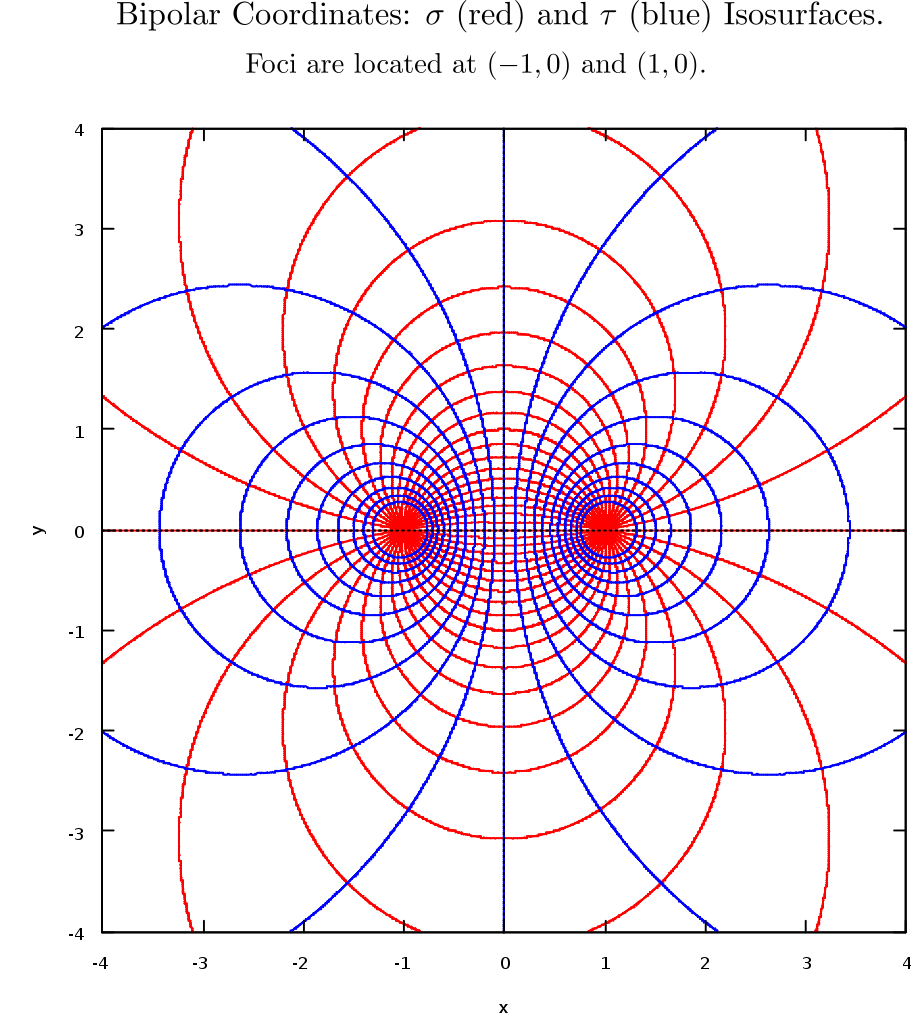
\includegraphics{src_plot/Bipolar.pdf}
\end{figure}

\paragraph{坐标曲线} % (fold)
\label{par:坐标曲线}

一组坐标曲线为$\pare{\pm a, 0}$两个焦点确定的Apollonius圆族, 另一组坐标曲线为与之正交的圆族.

% paragraph 坐标曲线 (end)

\paragraph{转换关系} % (fold)
\label{par:转换关系}

与平面直角坐标系有转换
\begin{align*}
    x &= a \frac{\sinh \tau}{\cosh \tau - \cos\sigma}, \\
    y &= a \frac{\sin\sigma}{\cosh\tau - \cos\sigma}.
\end{align*}
其中$\sigma = \angle F_1 P F_2$, $\tau = \ln F_1P/F_2P$, $F_1\pare{-a,0}$, $F_2\pare{a,0}$.

% paragraph 转换关系 (end)

\paragraph{度规} % (fold)
\label{par:度规}

\begin{align*}
    h_\sigma &= h_\tau = \frac{a}{\cosh \tau - \cos \sigma}, \\ \rd{A} &= \frac{a^2}{\pare{\cosh \tau - \cos\sigma}^2}\,\rd{\sigma}\,\rd{\tau}.
\end{align*}

% paragraph 度规 (end)

\paragraph{微分} % (fold)
\label{par:微分}

\begin{align*}
    \laplacian \Phi = \pare{\frac{\cosh \tau - \cos\sigma}{a}}^2 \pare{\frac{\partial^2\Phi}{\partial \sigma^2} + \frac{\partial^2\Phi}{\partial\tau^2}}.
\end{align*}

% paragraph 微分 (end)

\begin{figure}
    \centering
    \includegraphics{src_plot/testasy14+0.eps}
\end{figure}

% subsubsection 双极坐标系 (end)

% subsection 二维正交坐标系 (end)

% section 各种坐标系 (end)

\end{document}
